\chapter{船岸连接系统结构与分析}

船岸连接(Ship-to-Shore Connection),在不同的文献中名称也有不同的称呼,如冷熨烫(Cold Ironing)、岸侧电源(Shore-Side Electricity,SSE)、
岸电供电(Onshore Power Supply,OPS)、船舶岸电系统(Alternative Maritime Power Supplly,AMPS)。
虽然名称有所不同,但它们都涉及到停泊船舶靠港后关闭其船载辅助发动机,并使用港口提供的清洁能源为船载主要系统供电,
满足所有如照明、制冷和货物卸设施等船载设备的电力需求。这种技术允许停泊的船只使用船舶岸电,而不是依靠辅助发动机产生的
动力来减少港口的废气排放。

\section{船岸连接系统的组成}


船岸电力系统由岸基电力供应系统、船岸连接系统和船载电力接收系统组成。岸基电力系统结构的示意图如图1所示。
首先,将电网电压转换成低电压。随后,通过整流逆变器装置和变压器获得所需的板上电压。最后,岸电与船的连接应通过
连接桩进行。具体来说,岸基电源的供电系统主要是岸基变频电源,其结构包括整流器、逆变器等。船岸连接系统可应用
于不同电压等级和类型的船舶。大型远洋货轮采用高压岸电,散货船主要采用低压。连接主要是指岸上与船之间不间断的
电网连接,这是岸电系统研究的难点之一,也是本研究的重点。

如图\ref{fig:一种HSVC示意图}所示,它需要三个基本组件:岸侧电气系统和基础设施、电缆管理系统和船侧电气系统。
岸侧电气系统将高压变电站的电力传输到船舶附近的连接点,即终端的配电箱,以转换电压电平、转换频率、
以不间断的方式在船舶电力接收系统之间切换等。电缆管理系统包括连接岸侧连接点和船载受电设施的电缆和设施。
电缆连接设施必须满足快速连接和储存的要求,不使用时应存放在船上、岸上或驳船上。船侧电气系统是在原有船载配电
系统基础上增加的受电单元,包括电缆绞车、变压器及相关管理系统(陈等,2019)。船载电站的发电机按电压等级可分为
高压和低压。高压船载电站的电压等级包括11 kV、6.6kV(60Hz)和6kV(50Hz),低压船载电站的电压等级包括400V(50Hz)
和440伏(60赫兹)。

\begin{figure}[!htp]
	\centering
	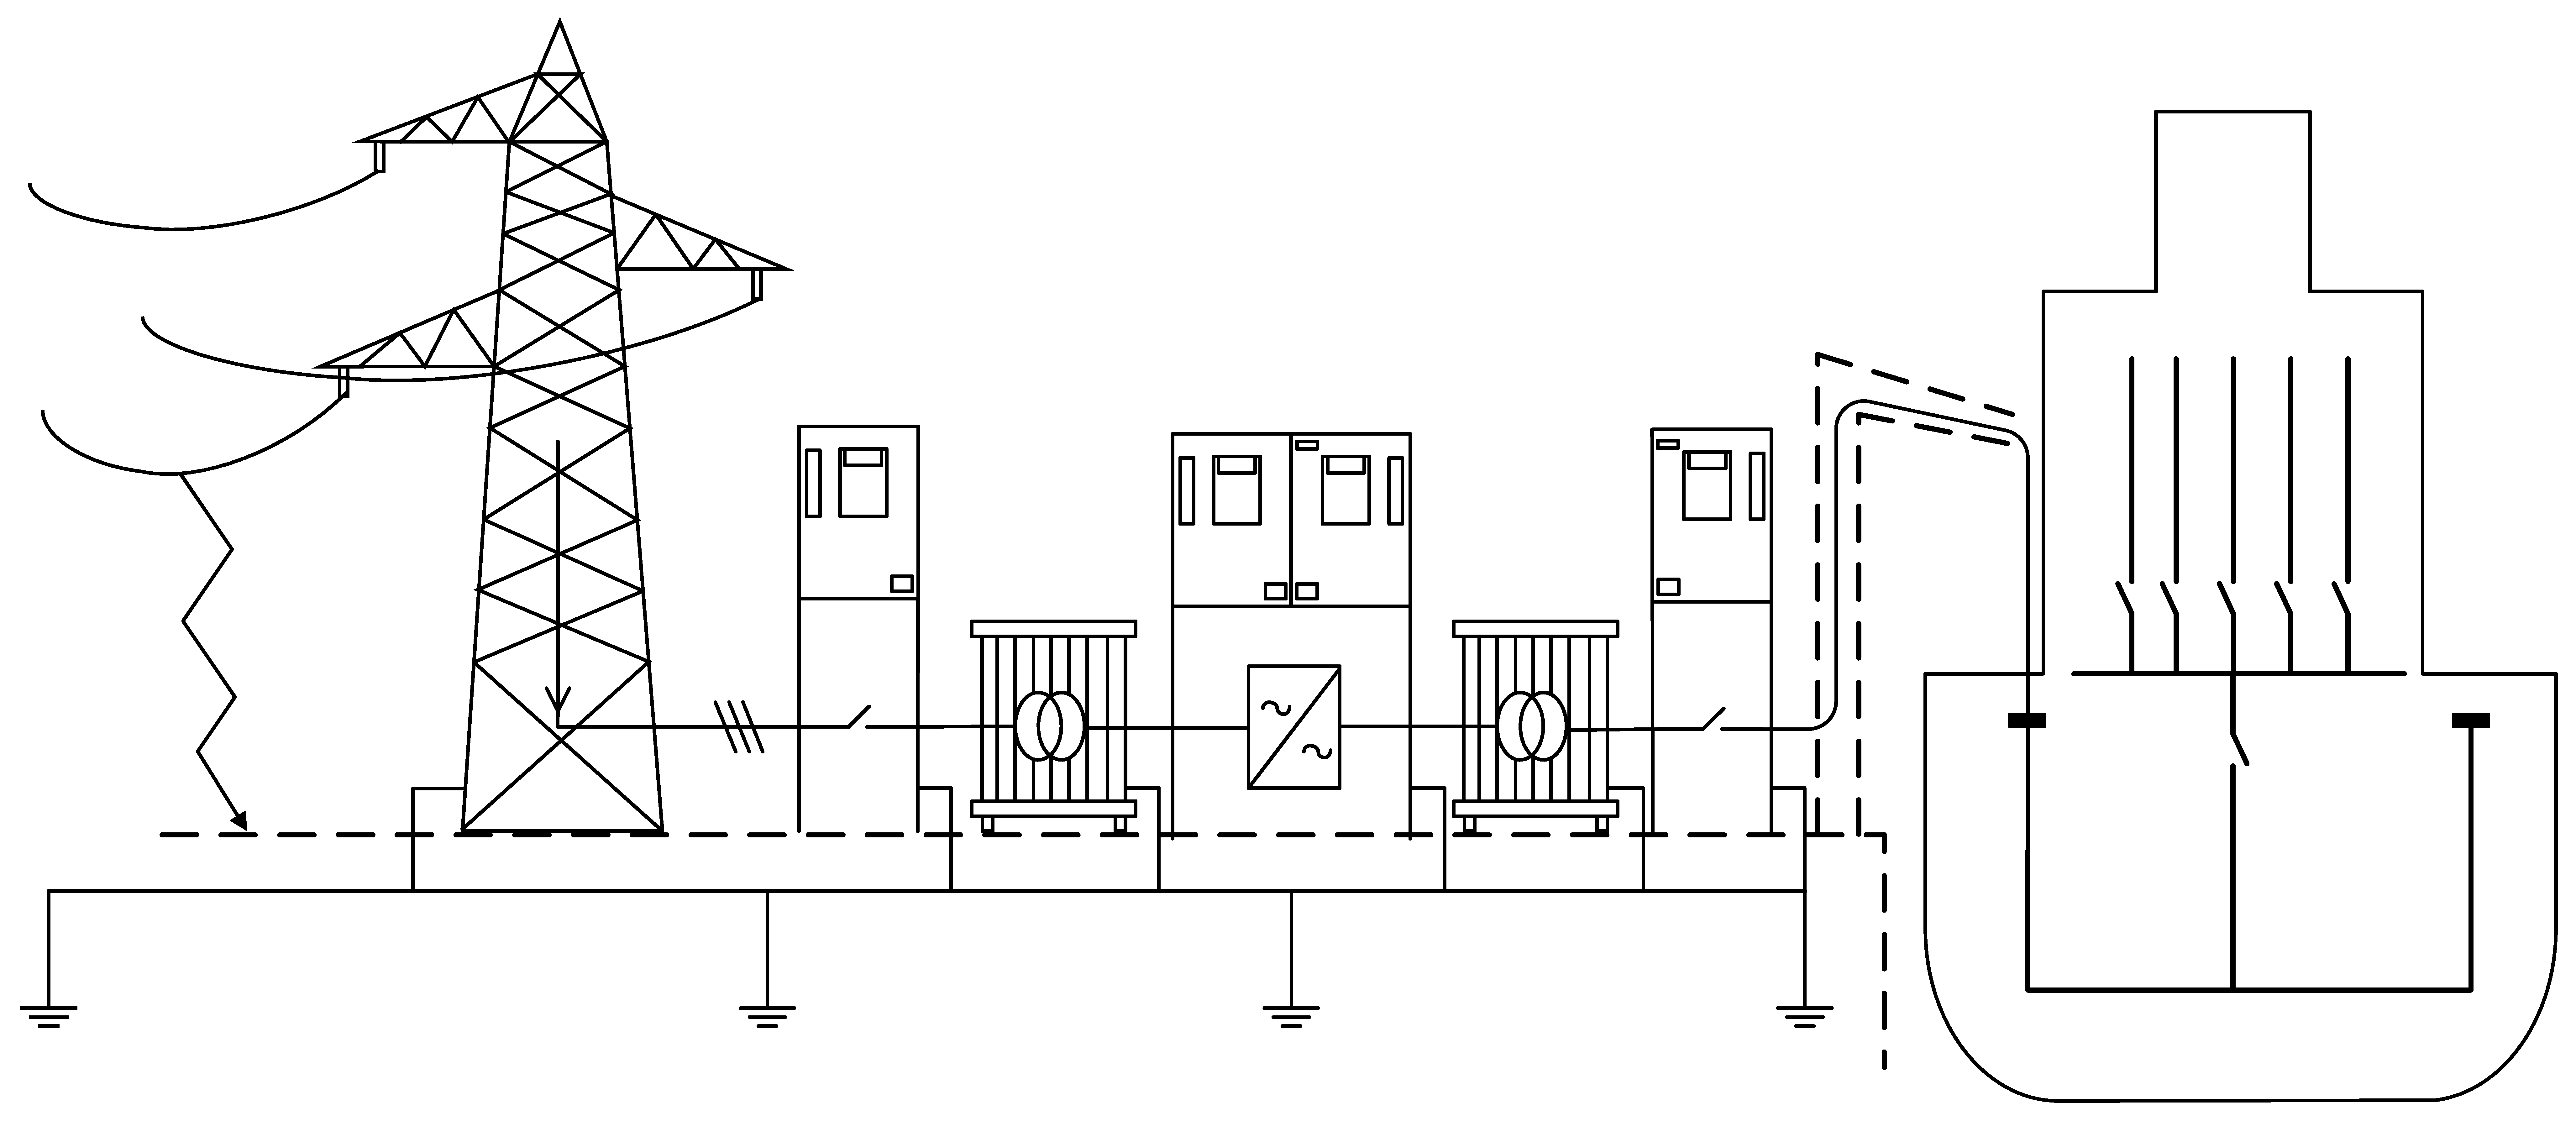
\includegraphics[width=0.95\textwidth]{高压船岸连接示意图.pdf}
	\caption{一种HSVC示意图}
	\label{fig:一种HSVC示意图}
\end{figure}

\begin{figure}[!htp]
	\centering
	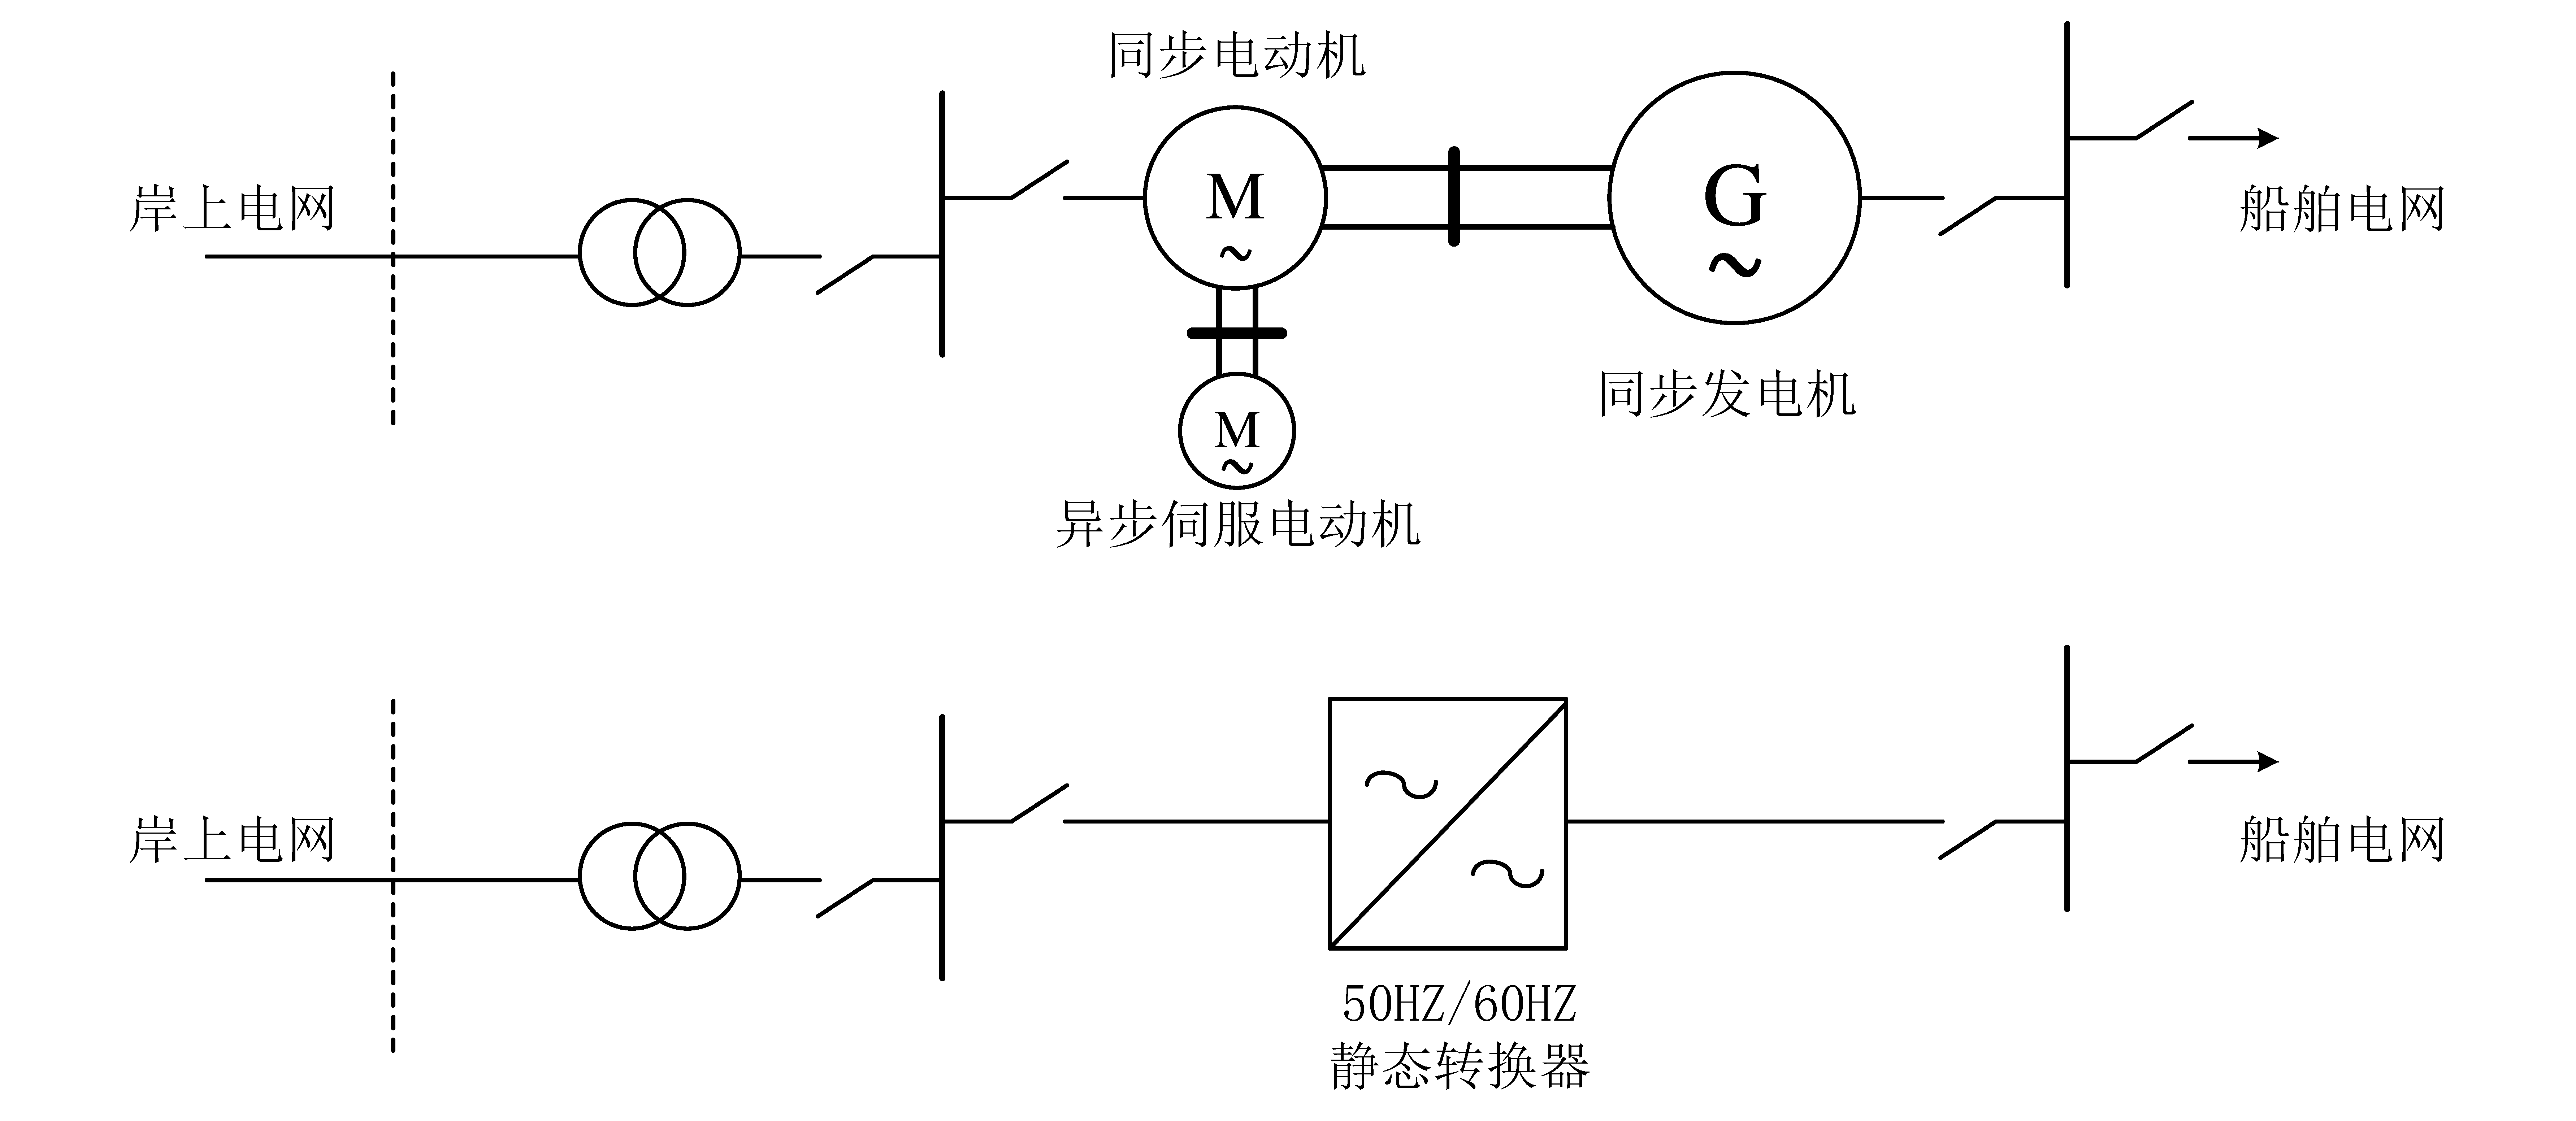
\includegraphics[width=0.85\textwidth]{旋转形态转换器对比.pdf}
	\caption{传统旋转变频与静态电源变频对比}
	\label{fig:传统旋转变频与静态电源变频对比}
\end{figure}

\section{船岸连接系统的配置方式}

\subsection{船岸连接高压岸电供电系统}

\zhlipsum[1]

\begin{figure}[!htp]
	\centering
	\includegraphics[width=0.9\textwidth]{高压岸电系统.pdf}
	\caption{高压岸电供电系统}
	\label{fig:高压岸电供电系统}
\end{figure}



\subsection{船岸连接低压岸电供电系统}


\zhlipsum[2]

\begin{figure}[!htp]
	\centering
	\includegraphics[width=0.9\textwidth]{低压岸电系统.pdf}
	\caption{低压岸电供电系统}
	\label{fig:低压岸电供电系统}
\end{figure}



\subsection{船岸连接小容量岸电供电系统}

\zhlipsum[3]

\begin{figure}[!htp]
	\centering
	\includegraphics[width=0.9\textwidth]{小容量岸电系统.pdf}
	\caption{小容量岸电供电系统}
	\label{fig:小容量岸电供电系统}
\end{figure}



\subsection{船岸连接不同方案对比}


% \begin{table}[!htp]
% 	\centering
% 	\caption[船用岸电供电方式比较]{船用岸电供电方式比较}
% 	\label{tab:船用岸电供电方式比较latex}
% 	\resizebox{\textwidth}{!}{%
% 	\begin{tabular}{cccc}  
% 	  \toprule
% 	    & 低压岸电/低压船舶     & 高压岸电/低压船舶        & 高压岸电/高压船舶  \\ 
% 	  \midrule
% 	  岸上系统电压/kV & 0.44          & 6~20             & 6.6/11     \\
% 	  船舶配电电压/kV & 0.44          & 0.4              & 6.6/11     \\
% 	  港口电网频率/Hz & 60            & 50               & 60         \\
% 	  船舶用电频率/Hz & 60            & 50               & 60         \\
% 	  岸电接入方式    & 港口提供电缆        & 港口提供电缆           & 船方提供电缆     \\
% 	  船舶改造复杂性   & 较小            & 较复杂,需要船舶上安装降压变压器 & 较小         \\
% 	  供电操作难易度   & 较复杂,需接驳船和多根电缆 & 较容易,仅需一根电缆       & 较容易,仅需少量电缆 \\
% 	  \bottomrule %添加表格底部粗线
% 	\end{tabular}
% 	}
% \end{table}


\zhlipsum[4]


\begin{table}[!htp]
	\centering
	\caption[船用岸电供电方式比较]{船用岸电供电方式比较}
	\label{tab:船用岸电供电方式比较}
	\resizebox{\textwidth}{!}{%
	\begin{tabular}{c}
		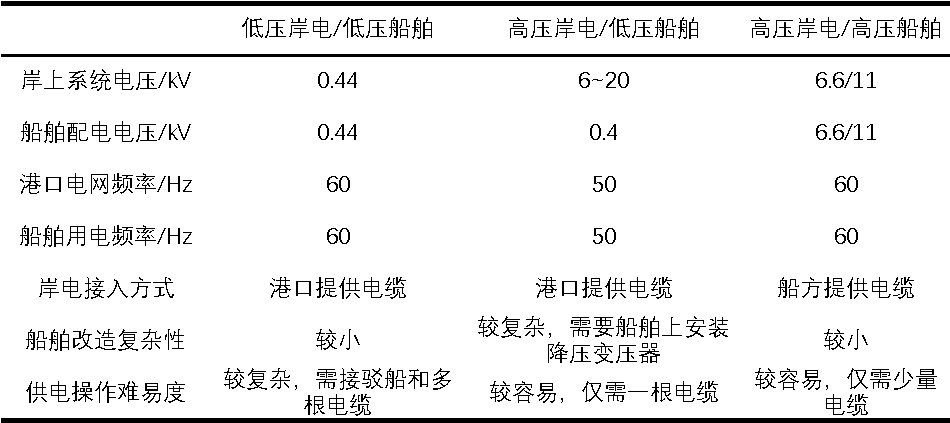
\includegraphics{船用岸电供电方式比较.pdf} 
	\end{tabular}
	}
\end{table}




\section{船岸连接系统面临的问题}
\subsection{船舶岸电供电并网切换}
船岸电力的电网连接是在船的柴油发电机和岸上电源之间。并网需要满足四个条件:船舶发电机的相序、幅值、相位、频率
必须与岸电一致。保持相同的相序尤为重要。影响瞬时电压差的三个因素是频率差、相位差和电压差。船岸自动准同步并网
的四个条件如下:
(1)船舶电源的相序必须等于岸上电源的相序;
(2)船舶电源的电压幅值必须等于岸上电源的电压幅值;
(3)船舶电源的频率必须等于岸上电源的频率;
(4)船舶电源的相位必须等于岸上电源的相位。
这些条件在理想情况下得到满足。事实上,相位、频率和振幅不可能同时完全一致。但只要船电和岸电的相位、频率、幅度差
在一定值内,涌流就在系统可接受的范围内,所以可以进行船岸并网。

\subsubsection{主动并网切换}
\subsubsection{被动并网切换}

\subsection{并网负载转移方式}
\subsection{逆功率处理方案}
\subsection{逆功率产生机理}
\subsection{逆功率的处理}
\subsection{不同控制方案简单对比}




\subsection{岸船连接段系统压降解决方案}

\subsubsection{隔离变压器的压降问题}
\subsubsection{输出电缆的压降问题}


\subsection{三相输出电压平衡控制技术}
\subsection{船岸等电位处理方案}


\zhlipsum[5]

\section{本章小结}


\zhlipsum[6]